\documentclass[10pt, letterpaper]{article}
\usepackage[english]{babel}
\usepackage[utf8]{inputenc}

% Adding images
\usepackage{graphicx}
\usepackage{subcaption}

% Adding links
\usepackage{hyperref}

\title{Homework Learning Agent}
\author{Calogero Carlino, 302154}
\date{December 19, 2024}

\begin{document}
\maketitle

\section{Introduction}
The code developed for this assignment includes modules for the 
implementations of the algorithms \texttt{ab\_minmax}, 
\texttt{bl\_minmax}, \texttt{bl\_minmax\_l},
\texttt{pred\_minmax}, \texttt{pred\_bl\_minmax} and 
\texttt{pred\_bl\_minmax\_l}.

The regressors for the predictive algorithms can be trained on two datasets \texttt{dataset.csv} and 
\texttt{extended\_dataset.csv}. The latter offers a more detailed state description. 
The methods for the generation of both datasets are inside
the \texttt{data\_analyst} module, while the regressor training session
functions are in the \texttt{trainer} module. The \texttt{oracle} module
on the other hand contains the wrapper functions for making predictions 
with the regressors in the predictive algorithms.

The game module for chess, on which these algorithms were tested and that 
implements the relevant state space definitions and functions 
(state space, possiblemoves(state)/neighborhood(state), final(state), H0 
static heuristic(s), function(s), ecc\dots) is the \texttt{chess\_game} module.

Lastly, in \texttt{main.py} there are several functions that make the algorithms play
with one another on a chess board. Each game is recorded by a Scorekeeper class
(defined in \texttt{corekeeper.py}) which will print some statistics in a \texttt{.json}
format alongside a \texttt{.txt} file that can be analyzed on \href{https://www.chess.com/analysis?tab=analysis}{chess.com}.

\section{Comparative statistics}
Each algorithm was tested with varying combinations of L, *l* and branch factor 
on the same randomly  generated boards.

The statistical data generated offers profound insights into the performance 
and characteristics of decision-making algorithms across varying conditions. 
By examining metrics such as heuristic evaluation levels (HL), computation time, 
and the H0 evaluation function, patterns emerge that illuminate the strengths 
and limitations of each approach.

The graphs shown in \emph{Picture \ref{fig:algorithms_comparisons}} were produced out of the test data.

\begin{figure}[h]
    \centering
    \begin{subfigure}[b]{0.475\textwidth}
      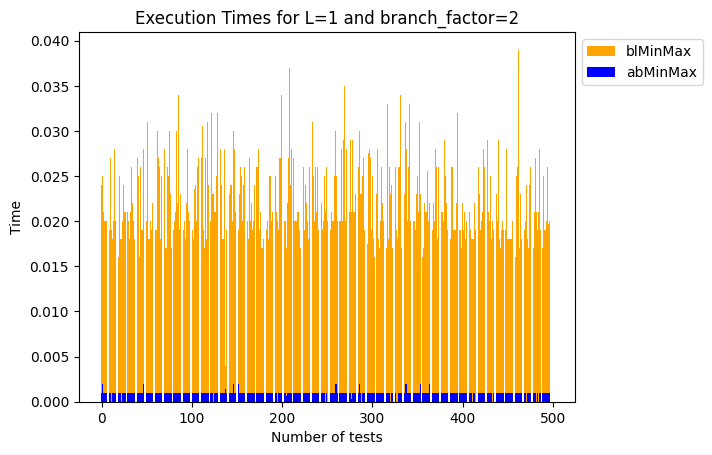
\includegraphics[width=\textwidth]{images/bl_minmax_vs_ab_minmax_execution_times_for_L1_and_bf2.png}
      \caption{blMinMax vs abMinMax execution time for L=1 and branch\_factor=2}
      \label{bl_minmax_vs_ab_minmax_execution_times_for_L1_and_bf2}
    \end{subfigure}
    \hfill
    \begin{subfigure}[b]{0.475\textwidth}
      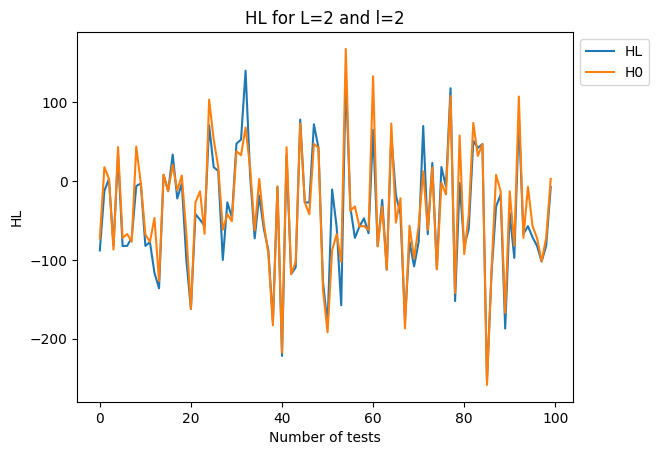
\includegraphics[width=\textwidth]{images/bl_minmax_l_different_choices_of_l_HL_for_L2_and_l2.png}
      \caption{blMinMaxl different choices of l HL values for L=2 and l=2}
      \label{bl_minmax_l_different_choices_of_l_HL_for_L2_and_l2}
    \end{subfigure}
    
    \medskip % create some *vertical* separation between the graphs
    
    \begin{subfigure}[b]{0.475\textwidth}
      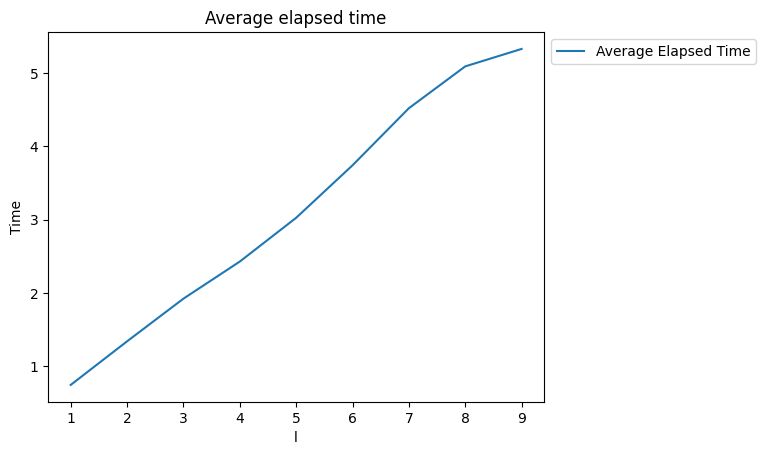
\includegraphics[width=\textwidth]{images/bl_minmax_l_optimal_l_with_L10_average_elapsed_time.png}
      \caption{blMinMaxl optimal l with L=10 average elapsed time}
      \label{bl_minmax_l_optimal_l_with_L10_average_elapsed_time}
    \end{subfigure}
    \hfill
    \begin{subfigure}[b]{0.475\textwidth}
      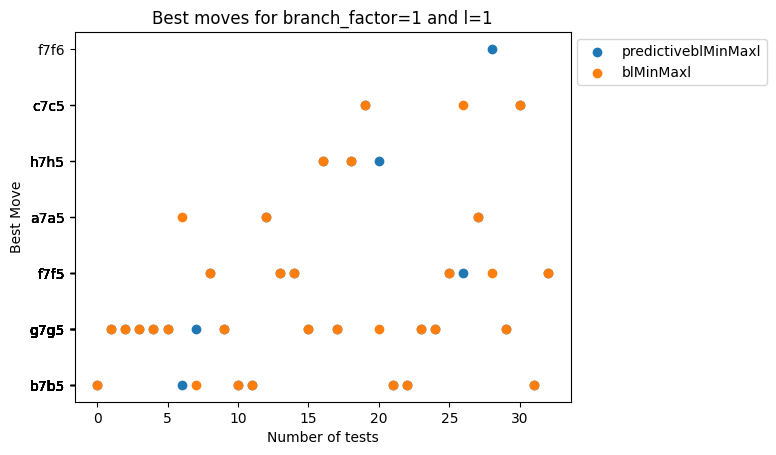
\includegraphics[width=\textwidth]{images/predictiveblMinMaxl_vs_blMinMaxl_best_moves_for_bf1_and_l1.png}
      \caption{predictiveblMinMaxl vs blMinMaxl Best moves for branch\_factor=1 and l=1}
      \label{predictiveblMinMaxl_vs_blMinMaxl_best_moves_for_bf1_and_l1}
    \end{subfigure}
    
    \caption{Graphs derived by testing maze runner algorithms 80 times in a room with increasing obstacles}
    \label{fig:algorithms_comparisons}
\end{figure}

\section{Conclusions}
The data and comparisons presented provide valuable insights into the suitability and performance of the different algorithms for specific scenarios, along with their trade-offs and optimal configurations.

The abMinMax algorithm emerges as a robust choice. Its ability to systematically explore all possible paths, coupled with alpha-beta pruning, ensures optimal decisions within computational limits. This method's efficiency, adaptability, and precision make it the superior option compared to its counterpart, blMinMax. On the other hand, blMinMax demonstrates reliability in simpler problems but lacks the dynamic pruning capabilities of abMinMax, which hampers its performance in more computationally demanding contexts.

The introduction of predictive capabilities, as seen in predMinMax, shifts the focus toward speed and adaptability. By relying on predictive models rather than exhaustive search, predMinMax significantly reduces computation time. However, this comes at the cost of guaranteed accuracy, as its decision-making heavily depends on the quality and reliability of its predictions.

The predictiveblMinMaxl algorithm provides a middle ground between exhaustive search and prediction-based decision-making. While predictiveblMinMaxl leverages predictions to handle larger decision trees efficiently, it does not guarantee optimal decisions. In contrast, blMinMaxl retains its reliability in deterministic problems by using learned evaluations without sacrificing accuracy.

The analysis of the effects of parameters such as L and *l* reveals important trends. Increasing the search depth L generally results in higher heuristic evaluation scores (HL), reflecting a more thorough assessment of the decision tree. However, this improvement comes with a significant increase in computational cost, especially in deeper searches. Similarly, larger values of *l* refine the evaluations, leading to better HL scores. Nonetheless, this improvement diminishes when L is small, indicating that the benefits of higher *l* depend on an adequate search depth.

Branching factor, on the other hand, has a relatively minor impact on computation time for abMinMax and blMinMax, indicating that these algorithms' performance is not heavily influenced by the complexity of the decision tree in this dataset. However, predictive algorithms such as predMinMax and predictiveblMinMaxl are more sensitive to branching, as their reliance on heuristic predictions amplifies the significance of accurate evaluations when the branching factor increases.

The training of regressors introduces another layer of complexity. The comparison between static H0-based regressor and the one trained with H0 function dataset shows that the latter predicts a broader range of heuristic values. However, the computational cost nearly doubles for H0-function-trained models due to the increased complexity of their input data. While static H0-based regressors are faster, the enriched data of H0-function-trained models enhances their potential to handle more nuanced scenarios.

In conclusion, abMinMax and blMinMax performance improves with deeper searches, particularly with L=5, where they leverage pruning and systematic evaluation to ensure robust outcomes. Predictive algorithms, including predMinMax and predictiveblMinMaxl, benefit from carefully tuned parameters such as L and *l*.

Finally, the choice between static and extended regressors depends on the problem's complexity. While static regressors excel in simpler scenarios, extended datasets allow for more comprehensive evaluations, making them invaluable in challenging or dynamic environments. This data underscores the importance of aligning algorithmic choices and parameter tuning with the specific requirements and constraints of the application domain.

\end{document}